
\subsection{Lato Server}
\label{sec:latoServer}

\begin{figure}[H]
	\centering
	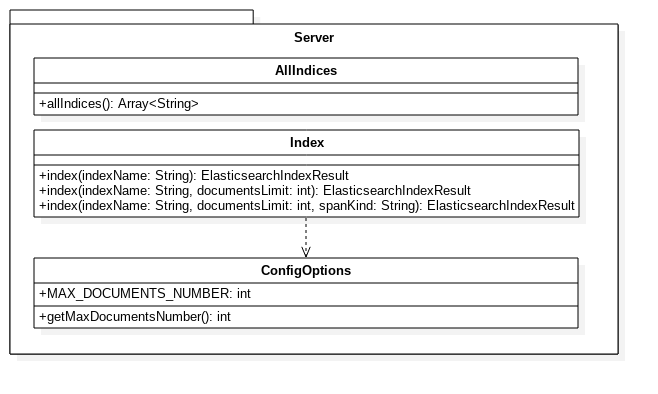
\includegraphics[width=1\textwidth]{Images/DiagrammaClassiServer.png}
	\caption{Diagramma UML delle classi riguardanti il lato server}
	\label{img:diagrammaClassiServer}
\end{figure}

\subsubsection{Generalità}
Il lato server si deve occupare di interrogare il database Elasticsearch ed esporre i risultati delle query tramite API REST al lato client. Le funzioni che il lato server può compiere sono \emph{volutamente}  poche e basilari. La scelta progettuale di spostare sul lato client tutta la parte di elaborazione del dato è stata dettata da necessità tecniche: il lato server di un plugin di Kibana viene eseguito all'interno di un'istanza del server Kibana. Spesso essi sono installati su server AWS con una limitata capacità di calcolo, molte volte 2GB di memoria RAM. Per questo motivo se avessimo eseguito elaborazioni complicate e impegnative su tali macchine ci sarebbe stato il rischio che con l'aumentare dell'utenza il servizio sarebbe potuto essere lento.

\subsubsection{Rappresentazione}
Nel seguente diagramma delle classi, figura \ref{img:diagrammaClassiServer}, le classi \texttt{AllIndices} e \texttt{Index} corrispondono all'interno del codice ad API esposte dal lato server al lato client. I metodi esposti intendono rappresentare il funzionamento della API. Ciascuna API è interrogabile dal lato client tramite una richiesta HTTP.


\subsubsection{Componenti}

\paragraph{ConfigOptions} \Spazio
È il componente che  contiene i parametri impostabili dal gestore del plugin per configurare il lato server. Consta di alcuni campi dati:

\begin{itemize}
	\item \texttt{MAX\_DOCUMENTS\_NUMBER: int} rappresenta il numero massimo di documenti che in una singola lettura vengono restituiti al chiamante. Questo limite è fondamentale poichè i documenti contenuti in un indice possono essere un numero \emph{molto} grande e se non si limita la quantità di dati restituiti il server potrebbe anche andare in stato di errore;
	
	\item \texttt{ELASTICSEARCH\_HOST\_IP: String} rappresenta l'indirizzo ip ospitante l'istanza di Elasticsearch;

	\item \texttt{ELASTICSEARCH\_HOST\_PORT: int} rappresenta la porta sulla quale è attiva l'istanza di Elasticsearch;
\end{itemize} 
Tutte le costanti vengono impostate al momento della creazione dell'oggetto \texttt{ConfigOptions}. I metodi sono: 
\begin{itemize}
	\item \texttt{getMaxDocumentsNumber(): int} che ritorna la costante appena descritta\\ \texttt{MAX\_DOCUMENTS\_NUMBER};
	\item \texttt{getElasticsearchHostIp(): String} che ritorna la stringa rappresentante l'indirizzo ip del server di Elasticsearch, salvata nella corrispondente costante;
	\item \texttt{getElasticsearchHostPort(): int} ritorna la porta sul quale è aperto il database Elasticsearch, salvata nella corrispondente costante; 
	\item \texttt{getElasticsearchHost(): String} ritorna la rappresentazione come stringa della combinazione dell'ip e della porta del database Elastisearch nella forma \texttt{'ip:porta'}, utilizzabile dalle route per collegarsi al database.
\end{itemize}

\paragraph{AllIndices} \Spazio
AllIndices è la API che si occupa di restituire al chiamante la lista di \emph{tutti} gli indici presenti all'interno della istanza di Elasticsearch collegata. La lista degli indici è un array di stringhe contenente per ogni indice il proprio nome.

\paragraph{Index} \Spazio
Index è la API che espone l'interfaccia per poter leggere i documenti contenuti all'interno di un indice. Nella richiesta GET deve essere specificato un parametro chiamato \texttt{index}, il cui valore rappresenta l'indice del quale si vogliono ottenere i dati. Ciò che viene ritornato al richiedente è un oggetto \emph{grezzo}, ovvero la risposta dell'istanza Elasticsearch, con tutti i dati amministrativi che Elasticsearch utilizza annessi (e.g. campi preceduti da underscore, \texttt{"\_id"}). Sarà compito del client reperire le informazioni a lui utili. L'oggetto ritornato è rappresentato con il tipo \texttt{ElasticsearchIndexResult}, che è descritto nella sezione \ref{sec:elasticsearchIndexResult} e rappresentato interamente nella Figura \ref{img:dati}.

È possibile inoltre specificare come parametri opzionali nella richiesta nel parametro\\ \texttt{documentsLimit} per richiedere un numero massimo di documenti. Comunque, se tale numero dovessere superare la soglia data da \texttt{ConfigOptions.getMaxDocumentsNumber()}, il numero massimo di documenti verrebbe impostato ad \texttt{ConfigOptions.getMaxDocumentsNumber()}. Se non si specifica \texttt{documentsLimit} il massimo di documenti ritornati sarà\\ \texttt{ConfigOptions.getMaxDocumentsNumber()}.
È anche possibile specificare un parametro opzionale chiamato \texttt{requestKind}, che può essere impostato a \texttt{Server} oppure \texttt{Database}, che ritorna solo documenti che nel campo \texttt{type} hanno tale valore. 
